\section{An example of the ODIN}

\begin{frame}{An example of the ODIN}
	\framesubtitle{Rigid body equation of motion}
	ODIN = Omni-directional intelligent navigation \footnote{Choi, Hyun-Taek, et al. "Development of an underwater robot, ODIN-III." Proceedings 2003 IEEE/RSJ International Conference on Intelligent Robots and Systems (IROS 2003)(Cat. No. 03CH37453). Vol. 1. IEEE, 2003.},\footnote{Ali, Nihad, Isaac Tawiah, and Weidong Zhang. "Finite-time extended state observer based nonsingular fast terminal sliding mode control of autonomous underwater vehicles." Ocean Engineering 218 (2020): 108179.}
	
	\begin{tikzpicture}[remember picture,overlay]
		% \node[fill=blue!30, text=white, font=\large, rounded corners] 
		\node at (current page.north east) [xshift=-3cm, yshift=-5.5cm] 
		{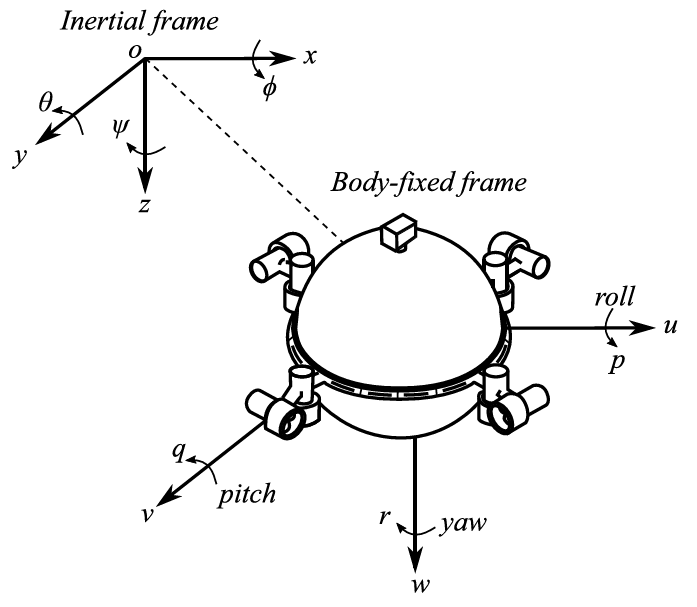
\includegraphics[width=0.4\linewidth]{img/ODIN.png}};
	\end{tikzpicture}
	
	\begin{tikzpicture}[remember picture,overlay]
		% \node[fill=blue!30, text=white, font=\large, rounded corners] 
		\node at (current page.north east) [xshift=-7cm, yshift=-5.5cm] 
		{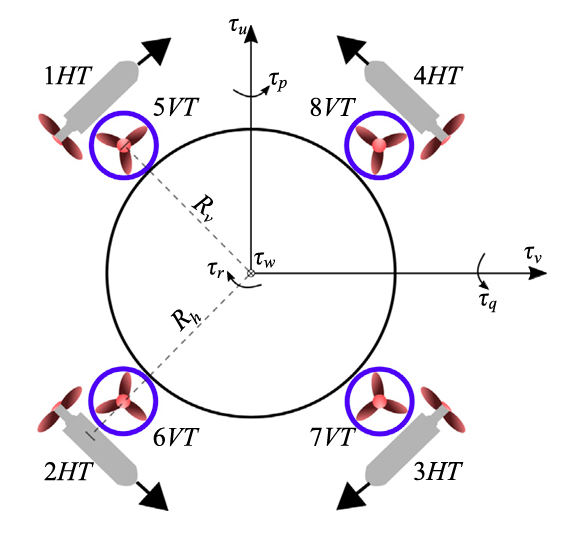
\includegraphics[width=0.25\linewidth]{img/ODIN1.png}};
	\end{tikzpicture}
	
	\begin{tikzpicture}[remember picture,overlay]
		% \node[fill=blue!30, text=white, font=\large, rounded corners] 
		\node at (current page.north east) [xshift=-11cm, yshift=-5.5cm] 
		{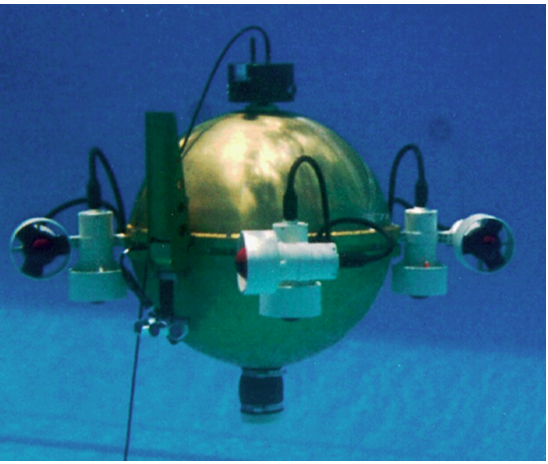
\includegraphics[width=0.25\linewidth]{img/ODIN2.png}};
	\end{tikzpicture}
\end{frame}




% =========================================
% =========================================




\begin{frame}{An example of the ODIN}
	\framesubtitle{Rigid body equation of motion}
	Dynamic equations
	\begin{align}
		M_{RB}\dot{\nu} + C_{RB}\nu = \tau_{RB}
	\end{align}
	where
	\begin{align}
		M_{RB} = \begin{bmatrix}
			mI_{3\times 3} & -mS(r_g^b) \\
			mS(r_g^b) & I_b
		\end{bmatrix}; C_{RB} = \begin{bmatrix}
			mS(\nu_2) & -mS(\nu_2)S(r_g^b) \\
			mS(\nu_2)S(r_g^b) & -S(I_b\nu_2)
		\end{bmatrix} \notag
	\end{align}
	Notice that, the term $C_{RB}(\nu)$ is modified by several mathematical transformations such as $C_{RB}(\nu) = C_{RB}(\nu_r)$ by linear velocity -independent parametrizations. Thus, the above dymanic equation could be represented as 
	\begin{align}
		M_{RB}\dot{\nu}_r + C_{RB}\nu_r = \tau_{RB}
	\end{align}
	with $\nu_r$ is the relative velocity of the vehicle. Therefore, the kinematics equation is represented as
	\begin{align}
		\dot{\eta} = J(\eta)\nu
	\end{align}
	where $J(\eta)$ is the Jacobian matrix.
\end{frame}



% =========================================
% =========================================




\begin{frame}{An example of the ODIN}
	\framesubtitle{Added mass}
	In order to lose the general, let's consider the ODIN as a spherical solid. Thus, the ODIN-geometry could be described as the following equation
	\begin{align}
		\dfrac{x^2}{a^2} + \dfrac{y^2}{b^2} + \dfrac{z^2}{c^2} = 0
	\end{align}
	Let's define \footnote{Lamb, Horace. Hydrodynamics. University Press, 1924.}
	\begin{align}
		\alpha_0 = abc \int_0^\infty \frac{\mathrm{d}\lambda}{(a^2 + \lambda) \, \Delta}, \quad
		\beta_0 = abc \int_0^\infty \frac{\mathrm{d}\lambda}{(b^2 + \lambda) \, \Delta}, \quad
		\gamma_0 = abc \int_0^\infty \frac{\mathrm{d}\lambda}{(c^2 + \lambda) \, \Delta}
	\end{align}
	with $\Delta = \big\{(a^2 + \lambda)(b^2 + \lambda)(c^2 + \lambda)\big\}^{\frac{1}{2}}$
	
	\textbf{Special case:} $a = b = c = R$, it is easy to achieve that 
	\begin{align}
		\alpha_0 = \beta_0 = \gamma_0 = R^3 \int\limits_0^\infty \frac{\mathrm{d}\lambda}{(R^2 + \lambda)^2\sqrt{(R^2 + \lambda)}} = R^3\dfrac{2}{3R^3} = \dfrac{2}{3}
	\end{align}
\end{frame}




% =========================================
% =========================================




\begin{frame}{An example of the ODIN}
	\framesubtitle{Added mass}
	Following \footnote{Imlay, Frederick H. The complete expressions for added mass of a rigid body moving in an ideal fluid. No. Report 1528. 1961.}, the added mass of the spherical-solid underwater vehicle could be represented as
	\begin{align}
		&X_{\dot{u}} = -\frac{\alpha_0}{2 - \alpha_0} \frac{4}{3} \pi \rho abc,\\
		&Y_{\dot{v}} = -\frac{\beta_0}{2 - \beta_0} \frac{4}{3} \pi \rho abc,\\
		&Z_{\dot{w}} = -\frac{\gamma_0}{2 - \gamma_0} \frac{4}{3} \pi \rho abc,\\
		&K_{\dot{p}} = -\frac{1}{5} \frac{(b^2 - c^2)(\gamma_0 - \beta_0)}{2(b^2 - c^2) + (b^2 + c^2)(\beta_0 - \gamma_0)} \frac{4}{3} \pi \rho abc,\\
		&M_{\dot{q}} = -\frac{1}{5} \frac{(c^2 - a^2)(\alpha_0 - \gamma_0)}{2(c^2 - a^2) + (c^2 + a^2)(\gamma_0 - \alpha_0)} \frac{4}{3} \pi \rho abc,\\
		&N_{\dot{r}} = -\frac{1}{5} \frac{(a^2 - b^2)(\beta_0 - \alpha_0)}{2(a^2 - b^2) + (a^2 + b^2)(\alpha_0 - \beta_0)} \frac{4}{3} \pi \rho abc.
	\end{align}
\end{frame}




% =========================================
% =========================================




\begin{frame}{An example of the ODIN}
	\framesubtitle{Added mass}
	\textbf{Special case:} $a = b = c = R$, then $\alpha_0 = \beta_0 = \gamma_0 = \dfrac{2}{3}$, therefore
	\begin{align}
		X_{\dot{u}} = Y_{\dot{v}} = Z_{\dot{w}} = -\rho\dfrac{2}{3}\pi R^3\\
		K_{\dot{p}} = K_{\dot{p}} = K_{\dot{p}} = 0
	\end{align}
	Written in matrix form,
	\begin{align}
		M_A = \begin{bmatrix}
			\rho\dfrac{2}{3}\pi R^3 I_3 & 0_3 \\ 0_3 & 0_3
		\end{bmatrix}
	\end{align}
	Then, it is easy to find the Coriolis term of added mass, which is not depended on $\nu_1$
	\begin{align}
		C_A(\nu_r) = \rho \frac{2}{3} \pi R^3
		\begin{bmatrix}
			0 & 0 & 0 & 0 & w_r & -v_r \\
			0 & 0 & 0 & -w_r & 0 & u_r \\
			0 & 0 & 0 & v_r & -u_r & 0 \\
			0 & w_r & -v_r & 0 & 0 & 0 \\
			-w_r & 0 & u_r & 0 & 0 & 0 \\
			v_r & -u_r & 0 & 0 & 0 & 0
		\end{bmatrix}
	\end{align}
\end{frame}



% =========================================
% =========================================




\begin{frame}{An example of the ODIN}
	\framesubtitle{Gravitational/buoyancy forces}
	Hydrostatics force of Submerged Vehicles is represented as
	\begin{align}
		g(\eta) =
		\begin{bmatrix}
			(W - B) \sin(\theta) \\
			- (W - B) \cos(\theta) \sin(\phi) \\
			- (W - B) \cos(\theta) \cos(\phi) \\
			- (y_g W - y_b B) \cos(\theta) \cos(\phi) + (z_g W - z_b B) \cos(\theta) \sin(\phi) \\
			(z_g W - z_b B) \sin(\theta) + (x_g W - x_b B) \cos(\theta) \cos(\phi) \\
			- (x_g W - x_b B) \cos(\theta) \sin(\phi) - (y_g W - y_b B) \sin(\theta)
		\end{bmatrix}
	\end{align}
	with $(x_g, y_g, z_g)$ and $(x_b, y_b, z_b)$ are the coordinates of CO and CB, respectively.
	
	\textbf{Special case:} 
	\begin{itemize}
		\item $W = B \to$ neutral buoyant, the Gravitational/buoyancy forces just cause the rotations (moments).
		\item $Oz_b$ and $Oz_g$ are coincidence. That mean $x_g = x_b$ and $y_g = y_b$. 
		\item  $CB \equiv CG \equiv CO$ and $W = B \to$ $g(\eta) = (0, 0, 0, 0, 0, 0)^\top$.
	\end{itemize}
\end{frame}



% =========================================
% =========================================




\begin{frame}{An example of the ODIN}
	\framesubtitle{Damping}
	Damping includes
	\begin{itemize}
		\item Linear damping 
		\begin{align}
			D = -diag(X_u, Y_v, Z_w, K_p, M_q, N_r)
		\end{align}
		\item Nonlinear term (important for high-speed vehicles)
		\begin{align}
			d(\nu_r) = \begin{bmatrix}
				\dfrac{1}{2}V_r^2S C_D(\alpha)\cos\alpha - \dfrac{1}{2}V_r^2S C_L(\alpha)\sin\alpha \\
				Y_{cross}\\
				-\dfrac{1}{2}V_r^2S C_D(\alpha)\sin\alpha - \dfrac{1}{2}V_r^2S C_L(\alpha)\cos\alpha \\
				0_{3\times 1}
			\end{bmatrix}
		\end{align}
		More details, $C_D$, $C_L$ are the drag, lifting coefficient, respectively.
		\begin{align}
			&F_{drag} = -\dfrac{1}{2}\rho V_r^2 S C_D(\alpha)\\
			&F_{lift} = -\dfrac{1}{2}\rho V_r^2 S C_L(\alpha)\\
			&Y_{cross} = -\dfrac{1}{2}\rho
			\int\limits_{-L/2}^{L/2}T(x)C_d^{2D}(x)|v_r + xr|(v_r + xr)dx
		\end{align}
		
		The sideslip angle ($\beta$) and attack angle ($\alpha$) is defined in slide \ref{slide: Transformation between BODY and FLOW}.
	\end{itemize}
\end{frame}


% =========================================
% =========================================



